\addcontentsline{toc}{chapter}{Next value prediction}
\chapter*{Next value prediction}

\addcontentsline{toc}{section}{Data Understanding}
\section*{Data Understanding}\label{Data Understanding}

~~ There are two sets of data one for training (train.csv) and one from testing (test.csv).

The datasets contain 3 different features: x, y and z components of acceleration collected every 10 seconds for a total of 144911 records. 

Here are the first few rows of the train dataset:

\begin{center}
\begin{tabular}{| c | c | c | c |} 
\hline
No. & x & y & z \\ [0.5ex] 
\hline
\hline
 0 & -24 & 749 & -626 \\
\hline
1 & -206 & 930 &  -63 \\
\hline
2 & -139 & 763 & -577 \\
\hline
3 & -503 & 441 & -557 \\
\hline
4 & -278 & 705 & -396 \\
\hline
5 &  240 & 839 & -310 \\
\hline
6 & -671 & 318 & -213 \\
\hline
7  & -45 & 296 & -927 \\
\hline
8 &  102 & 294 & -888 \\
\hline
9 &   15 & 635 & -671 \\ [1ex] 
\hline
\end{tabular}
\end{center}

Here is the time evolution of the three features over time:

\begin{figure}[H]
\centering
  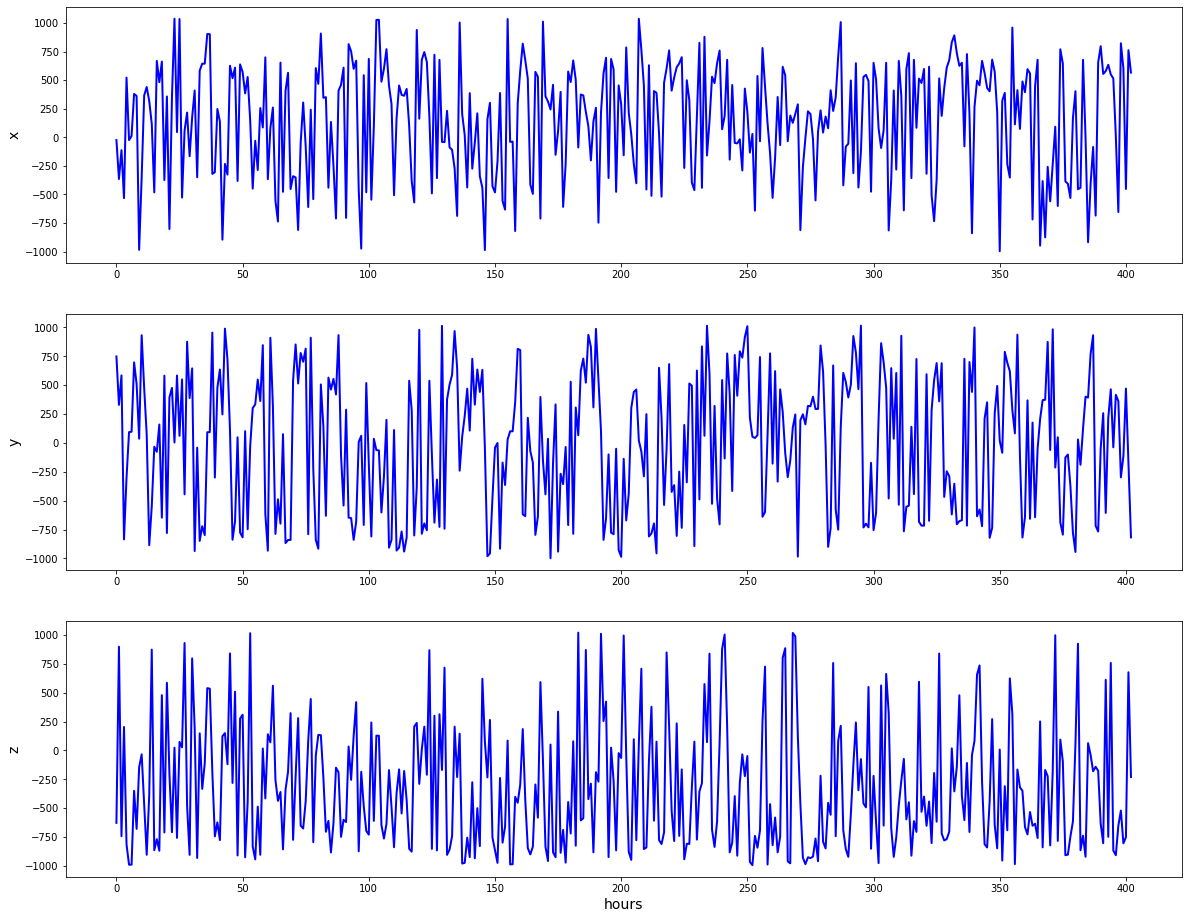
\includegraphics[scale=0.3]{img/task_1/data(hour).png}
  \caption{Time evolution of the three components of acceleration.}
  \label{fig: time evolution acc task 1}
\end{figure}

Let's take a look at the statistics of the dataset:

\begin{center}
\begin{tabular}{| c | c | c | c | c | c | c | c |} 
\hline
column & mean & std & min & 25\% & 50\% & 75\% & max \\ [0.5ex] 
\hline
\hline
x & 132.732967 & 491.697810 & -1239.0 & -291.0 & 214.0 & 539.0 & 1039.0 \\
\hline
y & -34.800146 & 594.977813 & -1019.0 & -646.0 & -14.0 & 466.0 & 1078.0 \\
\hline
z & -307.588768 & 538.335654 & -1001.0 & -794.0 & -416.0 & 83.0 & 1032.0 \\ [1ex]
\hline
\end{tabular}
\end{center}


\begin{figure}[H]
\centering
  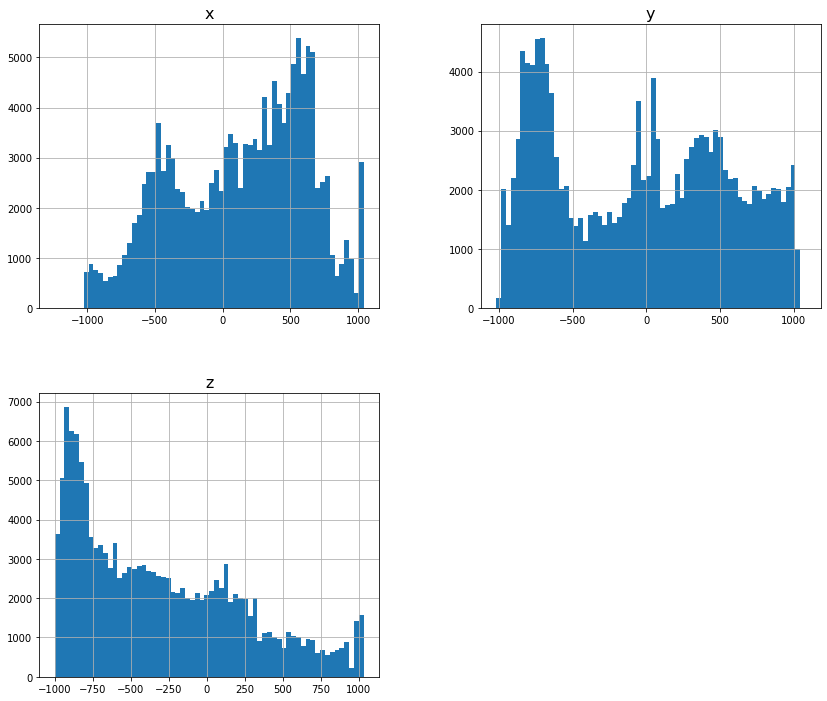
\includegraphics[scale=0.4]{img/task_1/histograms.png}
  \caption{Distribution of the data.}
  \label{fig: histograms task 1 }
\end{figure}



\addcontentsline{toc}{section}{Data Preparation}
\section*{Data Preparation}\label{Data Preparation}

\addcontentsline{toc}{subsection}{Splitting}
\subsection*{Splitting}\label{Splitting}

~~We'll use a 80\% of the train data (train.csv) for training and the remaining 20\% for validation. The test data (test.csv) was set aside for testing the model.

\begin{lstlisting}[language=Python]
import pandas as pd

train_data = pd.read_csv('train.csv', sep = ',')
test = pd.read_csv('test.csv', sep = ',')

n = len(train)

train = train_data[           : int(n*0.8)]
valid = train_data[int(n*0.8) :           ]
\end{lstlisting}

\addcontentsline{toc}{subsection}{Scaling}
\subsection*{Scaling}\label{Scaling}

~~We'll transform each feature individually such that it is in the given range on the training set, in our case between -1 and 1. This transformation is often used as an alternative to zero mean, unit variance scaling.

\begin{lstlisting}[language=Python]
from sklearn.preprocessing import MinMaxScaler

scaler = MinMaxScaler(feature_range=(-1,1))

train = scaler.fit_transform(train_df)
valid = scaler.transform(valid_df)
\end{lstlisting}

\addcontentsline{toc}{subsection}{Windowing}
\subsection*{Windowing}\label{Windowing}

~~Our model will make a set of predictions based on a window of consecutive samples from the data. The main features of the input windows are:

\begin{itemize}
  \item[1.] the window size (number of time steps) of the input and
  \item[2.] the window shift.
\end{itemize}

In this work we will make a single prediction 1 minute into the future, given 5 minutes of history. 

For the purpose of demonstration suppose that x has these values: x = [0, 1, 2, 3, 4]. Assume that the size of the window is 2 and the shift is 1. We create the following sequences: data = [[0, 1], [1, 2], [2, 3]], , label = [[2], [3], [4]], the goal is to predict for the sequence [0, 1] the value 2, for [1, 2] the value [3] and fot the sequence [2, 3] the value [4].


\begin{lstlisting}[language=Python]
def split(data, win_size=30, win_shift=6, offset=1):

  rows = np.arange(win_size, len(data) - win_shift - 1, win_shift)

  samples = np.zeros((len(rows), win_size, data.shape[-1]))
  targets = np.zeros((len(rows),))

  for j, row in enumerate(rows):
    samples[j] = data[j * win_shift: row]
    targets[j] = data[row: row + offset]

  return samples, targets
\end{lstlisting}





\addcontentsline{toc}{section}{Data Modeling}
\section*{Data Modeling}\label{Data Modeling}

~~Time series prediction problems are a difficult type of predictive modeling problem. Unlike regression predictive modeling, time series also adds the complexity of a sequence dependence among the input variables. A powerful type of neural network designed to handle sequence dependence is called Recurrent Neural Network (RNN). 

When reading a sentence the human brain processes it word by word while keeping memories of what came before; this gives humans a fluid representation of the meaning conveyed by the sentence. Biological intelligence processes information incrementally while maintaining an internal model of what it’s processing, built from past information and constantly updated as new information comes in.

A RNN adopts the same principle, albeit in an extremely simplified version: it processes sequences by iterating through the sequence elements and maintaining a state containing information relative to what it has seen so far. In effect, an RNN is a type of neural network that has an internal loop. The state of the RNN is reset between processing two different, independent sequences, so you still consider one sequence a single data point: a single input to the network. What
changes is that this data point is no longer processed in a single step; rather, the network internally loops over network: a network with a loop sequence elements.

Susch RNNs have a major issue: although it should theoretically be able to retain at time t information about inputs seen many timesteps before, in practice, such long-term dependencies are impossible to learn. This is due to the vanishing gradient problem, an effect that is similar to what is observed with non-recurrent networks (feedforward networks) that are many layers deep: as you keep adding layers to a network, the network eventually becomes untrainable. Long Short-Term Memory (LSTM) networks tackle this problem. LSTM network adds a way to carry information across many timesteps thus preventing older signals from gradually vanishing during processing. We will use this type of netkwork for modeling our data.

An important constructor argument for all Keras RNN layers, such as tf.keras.layers.LSTM, is the return\_sequences argument. This setting can configure the layer in one of two ways:

\begin{itemize}
  \item[1.] If False, the default, the layer only returns the output of the final time step, giving the model time to warm up its internal state before making a single prediction:
\end{itemize}


\begin{figure}[H]
\centering
  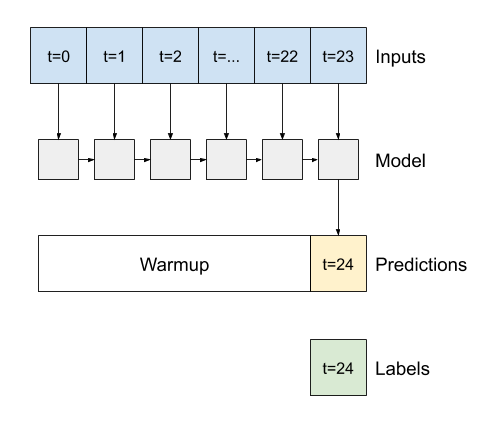
\includegraphics[scale=0.35]{img/task_1/fig1.png}
  \label{fig: }
\end{figure}


\begin{itemize}
  \item[1.] If True, the layer returns an output for each input. This is useful for:
  \begin{itemize}
     \item[a)] Stacking RNN layers.
     \item[b)] Training a model on multiple time steps simultaneously.
   \end{itemize}
\end{itemize}

\begin{figure}[H]
\centering
  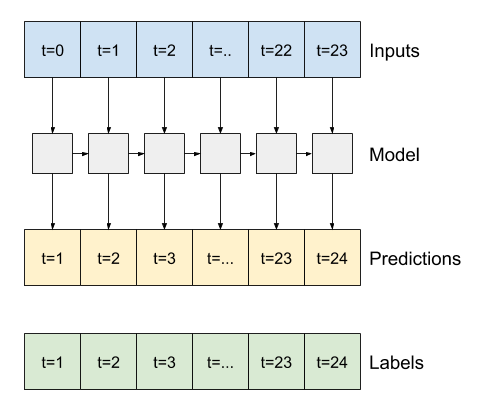
\includegraphics[scale=0.35]{img/task_1/fig2.png}
  \label{fig: }
\end{figure}


Here is our model.

\begin{lstlisting}[language=Python]
lstm = tf.keras.models.Sequential([
	tf.keras.layers.LSTM(16, 
		     input_shape=(sequence_length, numumber_of_features), 
		     return_sequences=True),
	tf.keras.layers.LSTM(8),
	tf.keras.layers.Dense(1, activation='tanh')
])
\end{lstlisting}

\begin{lstlisting}[language=Python]
lstm.compile(loss = 'mae', optimizer='adam')

history = lstm.fit(x_train, y_train, epochs=100, 
			validation_data=(x_valid, y_valid), 
			verbose = 1, batch_size=32, shuffle=False)
\end{lstlisting}

We obtain the fallowing results.

\begin{center}
\begin{tabular}{| c | c | c | c |} 
\hline
 & x & y & z  \\ [0.5ex] 
\hline
\hline
MAE & 54.55 & 59.22 & 61.74 \\
\hline
\end{tabular}
\end{center}

As mentioned before we use a window of 5 minutues and a shift of 1 minute, but this was an arbitrary choice. In order to evaluate the impact of window size and window shift we rerun our model varying this two parameters.

Mean Square Error (MAE) with a fixed window shift of 1 minute and variable window size. 

\begin{center}
\begin{tabular}{| c | c |} 
\hline
Window (min) & MAE  \\ [0.5ex] 
\hline
\hline
 1 & 65.14 \\
 \hline
 2 & 55.27 \\
 \hline
 3 & 63.99 \\
 \hline
 4 & 55.63 \\
 \hline
 5 & 60.96 \\
 \hline
 6 & 55.34 \\
 \hline
 7 & 63.05 \\
 \hline
 8 & 58.61 \\
 \hline
 9 & 55.33 \\
 \hline
 10 & 54.85 \\
 \hline
 11 & 54.47 \\
 \hline
 12 & 55.03 \\
 \hline
 13 & 58.72 \\
 \hline
 14 & 54.69 \\
 \hline
 15 & 64.59 \\
\hline
\end{tabular}
\end{center}

Mean Square Error (MAE) with a fixed window size of 5 minutes and variable window shift. 

\begin{center}
\begin{tabular}{| c | c |} 
\hline
Shift (min) & MAE  \\ [0.5ex] 
\hline
\hline
0.5 & 61.46\ \\
\hline
1 & 57.68\ \\
\hline 
1.5 & 57.92\ \\
\hline 
2 & 55.09 \\
\hline 
2.5 & 54.76\ \\
\hline 
3 & 54.62 \\
\hline 
3.5 & 58.28 \\
\hline 
4 & 57.29\ \\
\hline 
4.5 & 60.71 \\
\hline 
5 & 56.14 \\
\hline
5.5 & 59.64 \\
\hline 
6 & 55.21 \\
\hline
6.5 & 60.45 \\
\hline
7 & 58.58 \\
\hline 
7.5 & 53.86 \\
\hline
\end{tabular}
\end{center}

